%  latex main && dvips main && open -a preview main.ps
%  make slides
% rm main.aux main.log main.dvi main.nav main.out main.snm main.vrb main.toc modefile.aux 

\documentclass[dvips, % handout,
               xcolor=pst,
               hyperref={colorlinks=false,
%               hyperref={colorlinks=true,linkcolor=blue,urlcolor=blue,
               dvips,
               citecolor=magenta,menucolor=cyan,
               bookmarks,bookmarksopen,pdfpagemode=UseThumbs}
              ]{beamer}
\usepackage{etex}\reserveinserts{28} % important for extra package loading
\usepackage{amssymb}
\renewcommand{\le}{\leqslant}
\renewcommand{\ge}{\geqslant}
\usepackage{amsmath}
\usepackage{amsfonts}
\usefonttheme{professionalfonts} % keeps \boldsymbol working
\usepackage{wasysym}
\usepackage{fancyvrb}
\usepackage{calculator} % for the curve/gfx for function continuity
\usepackage{animate}
\usepackage{xfp} % for arithmetic - \fpeval


% From: http://tex.stackexchange.com/questions/66655/numbered-definitions-theorems-in-beamer
% You can set the theorems template with the numbered option:
% \setbeamertemplate{theorems}[numbered]
% or with the ams style option:
% \setbeamertemplate{theorems}[ams style] 
% If additionally you use the envcountsect class option by loading beamer in the following way:
% \documentclass[envcountsect]{beamer}
% then theorems, definitions, and so on to be numbered locally to each section (by default they are numbered consecutively throughout the presentation).
%\setbeamertemplate{theorems}[numbered]
%% SS commented the baove out on 31 October 2018


% see http://tex.stackexchange.com/questions/14364/cross-referencing-between-different-files
% for this next package - allows referencing across files.
\usepackage{xr}\externaldocument{../ma2730}

\usepackage{ifthen}
\usepackage{graphicx}
%%%\usepackage[pdftex]{graphicx}\usepackage{epstopdf}
\usepackage[normalem]{ulem} % fancy underlining - normalem restores {\em }
\usepackage{epsf,pstricks,pst-grad,pst-text,pst-node,pst-3d}
\usepackage{tikz,pgfplots}
\usepackage{multido}
\usepackage{euscript,stmaryrd,mathrsfs,calligra}
\usepackage{animate}
\usepackage{multimedia}
\usepackage{texdraw}
\everytexdraw{\drawdim mm \setunitscale 1 \linewd 0.15 \arrowheadtype t:F
\arrowheadsize l:2 w:1 \normallines}
\def\zerolines{\linewd 0.0 }
\def\thinlines{\linewd 0.05 }
\def\normallines{\linewd 0.15 } % as above
\def\thicklines{\linewd 0.25 }
\def\verythicklines{\linewd 0.5 }
\def\TDblack{\writeps{0 0 0 setrgbcolor}}
\def\TDblue{\writeps{0 0 1 setrgbcolor}}
\def\TDred{\writeps{1 0 0 setrgbcolor}}
\def\TDgreen{\writeps{0 0.7 0 setrgbcolor}}

\usepackage{xfrac} % for \sfrac{2}{3} etc

\newcommand{\textbs}{{\char`\\}} % used for backslash in LaTeX notes
\renewcommand{\le}{\leqslant}\renewcommand{\ge}{\geqslant}
\newcommand{\Real}{\mathbb{R}}
\newcommand{\Natural}{\mathbb{N}}
\newcommand{\Integer}{\mathbb{Z}}
\newcommand{\Rational}{\mathbb{Q}}
\newcommand{\Complex}{\mathbb{C}}
\newcommand{\xref}[1]{\textup{(\ref{#1})}}
% Steve Noble's macros, for improper integrals
\newcommand{\dx}{\, \mathrm{d}x}
\newcommand{\du}{\, \mathrm{d}u}
\newcommand{\dr}{\, \mathrm{d}r}
\newcommand{\dt}{\, \mathrm{d}t}
\newcommand{\dy}{\,\mathrm{d}y}
\newboolean{bw}
\setboolean{bw}{false}
\ifthenelse{\boolean{bw}}
{\newcommand{\emphy}{\emph}
\renewcommand{\red}{}
\renewcommand{\blue}{}}{\newcommand{\emphy}{}}
\newenvironment{bsoln}{\textit{Bad Solution:}}{}
\newcounter{lcount}
\newenvironment{alist}
{\begin{list}{(\alph{lcount})}{\usecounter{lcount}\settowidth{\leftmargin}{(a)}
\addtolength{\leftmargin}{\labelsep}
}}{\end{list}}
\newtheorem{exercise}{Exercise}
\newtheorem{soln}{Solution}
%%%%%%%%%%%%%%%%%%%%%%%%%%%%%%%%%%%%%%%%%%%%%%%%%%%%%%%%%%%%%%
%%%% \ballref{stuff} puts stuff in little ball like in beamer lists; useful for numbering when it's not in an enumerate.
\beamertemplateballitem
\newcommand{\ballref}[1]{\begin{pgfpicture}{-1ex}{-0.65ex}{1ex}{1ex}
    \usebeamercolor[fg]{item projected}
{\pgftransformscale{1.75}\pgftext{\normalsize\pgfuseshading{bigsphere}}}
    {\pgftransformshift{\pgfpoint{0pt}{0.5pt}}
      \pgftext{\usebeamerfont*{item projected}#1}}
  \end{pgfpicture}}%
%%%%%%%%%%%%%%%%%%%%%%%%%%%%%%%%%%%%%%%%%%%%%%%%%%%%%%%%%%%%%

% End of Steve's macros


\DeclareGraphicsRule{.ps.gz}{eps}{.ps.bb}{`gunzip -c #1}
\DeclareGraphicsRule{.eps.gz}{eps}{.eps.bb}{`gunzip -c #1}

% \includegraphics looks for pictures in these subdirectories:
\graphicspath{%
              {/home/Dropbox/gfx/}
              {/home/Dropbox/}
              % mac
              {/Users/simon/Dropbox/gfx/}
              {/Users/simon/Dropbox/}
              {/Users/simon/SkyDrive/}
              % Virtual Box, mint
              {/home/icsrsss/data/Dropbox/gfx/}
              {/home/icsrsss/data/Dropbox/}
              {/home/icsrsss/data/OneDrive/}
% 
%               {/home/icsf/icsrsss/Dropbox/gfx/}{/home/Dropbox/gfx/}{/Users/simon/Dropbox/gfx/}
%               {/home/icsf/icsrsss/}
%               {/home/icsf/icsrsss/webhome/LaTeX2e/talk/beamer/talks/gfx/}
%               {/home/icsf/icsrsss/webhome/LaTeX2e/gfx/}
%               {/home/icsf/icsrsss/webhome/LaTeX2e/papers/analysis/gfx/}
%               {/home/icsf/icsrsss/webhome/LaTeX2e/proposal/word/arteries2/gfx/}
              {..}{../gfx/}{./gfx/}}

\DeclareGraphicsRule{.eps.gz}{eps}{.eps.bb}{`gunzip -c #1}

%\usetheme{Warsaw}
%\usetheme{Madrid}
%\usetheme{Moscow}
%\usetheme{Bergen}
%\usetheme{Boadilla} % - not bad, quite minimal
%\usetheme{AnnArbor}
%\usetheme{CambridgeUS}
%\usetheme{Pittsburgh}
%\usetheme{Rochester}
%\usetheme{Antibes}
%\usetheme{JuanLesPins}
%\usetheme{Montpellier}
%\usetheme{Berkeley}
%\usetheme{PaloAlto}
%\usetheme{Goettingen}
%\usetheme{Marburg}
%\usetheme{Hannover}
%%%%%% \usetheme{Berlin}
%    \useinnertheme[shadow]{rounded}\useoutertheme{smoothbars}
    \useinnertheme{rounded}\useoutertheme{smoothbars}
%    \usecolortheme{beetle}
%    \usecolortheme{rose}
%    \usecolortheme{dolphin}
% These are OK
%    \usecolortheme{crane}
%    \usecolortheme{beaver} % OK, but suppresses part of the footline
%    \usecolortheme{dove} % very plain
%    \usecolortheme{dolphin} % harsh
%%%%%%%%%%    \usecolortheme{seahorse} % my usual blue
%    \usecolortheme{seagull} % colours get lost
%\usetheme{Ilmenau}
\setbeamertemplate{navigation symbols}{} % turn off smart board symbols
\setbeamertemplate{footline}
         {\quad\copyright\, Simon Shaw (2021)}

%\titlegraphic{\includegraphics[angle=45,width=1.0cm]{mesh0.007.eps}}

% allow \changemode{beamer}, \changemode{handout}
\makeatletter
\newcommand\changemode[1]{%
  \gdef\beamer@currentmode{#1}}
\makeatother

\newrgbcolor{darkgreen}{0.0 0.6 0.0}


\title[Python for Mathematics]
      {Introduction to Python for Mathematics\\ A Crash Course}
\subtitle[beamer]{}
\institute[Maths]
          {Mathematics}
\author[Shaw]{Simon Shaw
%\\  variationalform {@} Here and Now Learning
}

\date{\today}

% reactivate for final version - it is a very slow load otherwise.
% \logo{\includegraphics[width=0.75cm,angle=0]{logos/4862BICOMlogo-copy/logo/eps/4862_BICOM_Logo_Final_CMYK_outline.eps}}

%\setbeamercovered{transparent}
\setbeamercovered{dynamic} 

\begin{document}
%\setbeamercovered{transparent}
\begin{frame}
\titlepage
\end{frame}

%\changemode{beamer}
\include{modefile} % can contain one line: \changemode{handout}
\newcommand{\BoardworkColour}{\relax}


%  - - - - - - - - - - - - - - - - - - - - - - - -      FRAME
\begin{frame}[fragile]\frametitle{Contents}

\begin{itemize}

\item Anaconda and Jupyter

\item Leontief Input-Output Problems in Economics

\item 2D Plotting

\item Anonymity

\end{itemize}

\end{frame}
% - - - - - - - - - - - - - - - - - - - - - - - - - - - -



\section{Section 1: Anaconda and Jupyter}

%  - - - - - - - - - - - - - - - - - - - - - - - -      FRAME
\begin{frame}[fragile]\frametitle{Getting started}

\begin{itemize}

\item Log In

\item Start Anaconda Navigator (use search box)

\item untick box, click OK, or whatever you choose.

\item Press 'LAUNCH' for jupyter notebook (not jupyter lab)

\item Choose 'python 3' from 'new' menu on right

\item In  the first cell type \verb|2+3| followed by 
SHIFT-RETURN.
\end{itemize}

Did you get 5?

\end{frame}
% - - - - - - - - - - - - - - - - - - - - - - - - - - - -


\section{Section 2: I/O Problems}


%  - - - - - - - - - - - - - - - - - - - - - - - -      FRAME
\begin{frame}[fragile]\frametitle{}

\vfill
\begin{center}
\LARGE\blue

Leontief Input-Output

Problems in Economics

\end{center}
\vfill

\end{frame}
% - - - - - - - - - - - - - - - - - - - - - - - - - - - -

%  - - - - - - - - - - - - - - - - - - - - - - - -      FRAME
\begin{frame}[fragile]\frametitle{}

\begin{block}{Input Output Problems in Economics}
Consider the tourist economy in a small resort. The major industries are

\pause
\begin{description}[<+->]

\item[A: Accommodation] --- rentals, hotels, B \& B's, \ldots
\item[F: Food \& Drink] --- restaurants, kiosks, pubs, take away, \ldots
\item[E: Entertainment] --- theatre, cinema, nightclubs, \ldots
\item[T: Transportation] --- buses, trains, taxis, ferries, \ldots

\end{description}

\pause
The turnover of each of these industries will contain cash inputs from thenselves
and the others, as well as from external demand like tourists, other industrial
and commercial sectors, etc.

\end{block}

\pause
\begin{small}
\begin{block}{Reference}
\textit{Mathematics for Economics and Business},
Ian Jacques, Prentice Hall, 4 ed. 2003.
\end{block}
\end{small}

\end{frame}
% - - - - - - - - - - - - - - - - - - - - - - - - - - - -

%  - - - - - - - - - - - - - - - - - - - - - - - -      FRAME
\begin{frame}[fragile]\frametitle{Let's consider just A and F. Suppose  that \ldots}

\pause
Each \pounds 1 of A's turnover requires an input of 10p of its own turnover plus
30p of F's.

\medskip
\pause
Each \pounds 1 of F's turnover requires an input of 20p of its own turnover plus
50p of A's.

\pause
\medskip
So, assuming these proportions are constant across all turnover levels, if
we want A to turn over \pounds 50,000 and F to turnover \pounds 40,000 then:

\pause
\begin{description}[<+->]

\item[For A:] \pounds 50,000 requires \pounds 5000 (0.1 of \pounds 50,000) from
itself, plus \pounds 15,000 (0.3 of \pounds 50,000) from F. 

\item[For F:]  \pounds 40,000 requires \pounds 20,000 (0.5 of \pounds 40,000)
from A, plus \pounds 8000 (0.2 of \pounds 40,000) from itself.

\end{description}

\pause
Get the idea? Easily generalised to more industries. 
\pause {\red Look carefully:}

\pause\medskip
{\blue You can see matrices at work here}.
\pause {\red Let's figure it out\ldots}

\end{frame}
% - - - - - - - - - - - - - - - - - - - - - - - - - - - -

%  - - - - - - - - - - - - - - - - - - - - - - - -      FRAME
\begin{frame}[fragile]\frametitle{Look at it mathematically\ldots}

Each \pounds 1 of A's turnover requires an input of 10p of its own turnover plus
30p of F's.

\medskip
Each \pounds 1 of F's turnover requires an input of 20p of its own turnover plus
50p of A's.

\pause\medskip
{\blue Let $x_1$ denote A's turnover and $x_2$ denote F's turnover.}

\pause\medskip
{\red Also $d_1$ (resp. $d_2$) denote external demand for A (resp. F).}
Then:

\pause
\begin{align*}
x_1 & = \overbrace{0.1 x_1 + 0.5 x_2 + d_1}^{\text{payments to A}}
\\
\pause
x_2 & = \underbrace{0.3 x_1 + 0.2 x_2 + d_2}_{\text{payments to F}}
\end{align*}

\pause
{\red Can you see the matrix now?}

\end{frame}
% - - - - - - - - - - - - - - - - - - - - - - - - - - - -

%  - - - - - - - - - - - - - - - - - - - - - - - -      FRAME
\begin{frame}[fragile]\frametitle{Leontief's input-output model}

Let $x_1$ denote A's turnover and $x_2$ denote F's turnover.

\medskip
Let $d_1$ (resp. $d_2$) denote external demand for A (resp. F).
Then:
\begin{align*}
x_1 & = 0.1 x_1 + 0.5 x_2 + d_1
\\
x_2 & = 0.3 x_1 + 0.2 x_2 + d_2
\end{align*}

\pause
This can be written as
$\boldsymbol{x} = \boldsymbol{A}\boldsymbol{x}+\boldsymbol{d}$
for
\[
\boldsymbol{x} = \left(\begin{array}{r}
x_1 \\ x_2
\end{array}\right),
\qquad
\boldsymbol{d} = \left(\begin{array}{r}
d_1 \\ d_2
\end{array}\right)
\qquad\text{ and }\qquad
\boldsymbol{A} = \left(\begin{array}{rr}
0.1 & 0.5 \\ 0.3 & 0.2
\end{array}\right).
\]
\pause
In this model $\boldsymbol{A}$ is called the {\red matrix of technical coeffcients}, or 
the {\blue technology matrix}. (Developed by Wassily Leontief.)

\pause\medskip
$\boldsymbol{A}$'s columns give the inputs needed for one unit of output.

\end{frame}
% - - - - - - - - - - - - - - - - - - - - - - - - - - - -

%  - - - - - - - - - - - - - - - - - - - - - - - -      FRAME
\begin{frame}[fragile]\frametitle{Using the model}
The Leontief input-output model 
\[
\boldsymbol{x} = \boldsymbol{A}\boldsymbol{x}+\boldsymbol{d}
\]
can be used to answer three key questions:

\pause
\begin{enumerate}[<+->]

\item
Given total output $\boldsymbol{x}$, how much is available for demand $\boldsymbol{d}$?

\item[\ ]{\red Find  $\boldsymbol{d} = (\boldsymbol{I}-\boldsymbol{A})\boldsymbol{x}$}

\item
How much total output $\boldsymbol{x}$ is required to satisfy a given level of
demand $\boldsymbol{d}$?

\item[\ ]{\red Solve  $(\boldsymbol{I}-\boldsymbol{A})\boldsymbol{x} = \boldsymbol{d}$}

\item
How should output $\boldsymbol{x}$ change if demand changes by $\Delta\boldsymbol{d}$?

\item[\ ]{\red Solve  $(\boldsymbol{I}-\boldsymbol{A})\Delta\boldsymbol{x} = \Delta\boldsymbol{d}$}

\end{enumerate}

\pause
We'll do these by hand first, and then with python.

\pause
Remember that
${a\ b\choose c\ d}^{-1} = \frac{1}{\mathrm{det}}{\ \ d\ -b\choose -c\ \ \ a}$

\end{frame}
% - - - - - - - - - - - - - - - - - - - - - - - - - - - -

%  - - - - - - - - - - - - - - - - - - - - - - - -      FRAME
\begin{frame}[fragile]\frametitle{}
Use $\boldsymbol{x} = \boldsymbol{A}\boldsymbol{x}+\boldsymbol{d}$ with
$\boldsymbol{A}={0.1\ 0.5\choose 0.3\ 0.2}$ to answer these:

\bigskip

\begin{enumerate}[<+->]

\item
Given total output $\boldsymbol{x}={50000\choose 40000}$, how much is available for demand $\boldsymbol{d}$?

\item[\ ]{\red Find  $\boldsymbol{d} = (\boldsymbol{I}-\boldsymbol{A})\boldsymbol{x} =
{\ \ 0.9\ -0.5\choose -0.3\ \ 0.8}{50000\choose 40000} = {25000 \choose 17000}$}

\item
How much total output $\boldsymbol{x}$ is required to satisfy a given level of
demand $\boldsymbol{d} = {35000\choose 29000}$?

\item[\ ]{\red Solve  $(\boldsymbol{I}-\boldsymbol{A})\boldsymbol{x} = \boldsymbol{d}
\Longrightarrow
\boldsymbol{x} = \frac{10}{57}{8\ \ 5 \choose 3\ \ 9}{35000\choose 29000}
\approx { 74561 \choose 64210}$}

\item
How should output $\boldsymbol{x}$ change if demand changes by $\Delta\boldsymbol{d}= {2500\choose 1900}$?

\item[\ ]{\red Solve  $(\boldsymbol{I}-\boldsymbol{A})\Delta\boldsymbol{x} = \Delta\boldsymbol{d}
\Longrightarrow
\boldsymbol{\Delta x} = \frac{10}{57}{8\ \ 5 \choose 3\ \ 9}{2500\choose 1900}
\approx { 5175 \choose 4315}$}

\end{enumerate}

\bigskip

Now let's do this in python\ldots

\end{frame}
% - - - - - - - - - - - - - - - - - - - - - - - - - - - -

%  - - - - - - - - - - - - - - - - - - - - - - - -      FRAME
\begin{frame}[fragile]\frametitle{The key commands}

{\footnotesize\blue
\begin{verbatim}
import numpy as np                      # import numerical python
A = np.array([[0.1, 0.5],[0.3, 0.2]])   # our technology matrix
Id = np.eye(2)                          # 2 by 2 identity matrix
d = np.array([[35000],[29000]])         # demand vector d
print(np.linalg.solve(Id-A, d))         # solve (I-A) x = d for x
Dd = np.array([[2500],[1900]])          # change in demand vector, Dd
print(np.linalg.solve(Id-A, Dd))        # solve (I-A) Dx = Dd for Dx
\end{verbatim}
}

Note you can start a new cell whenever you like.

\medskip
Do so frequently.

\end{frame}
% - - - - - - - - - - - - - - - - - - - - - - - - - - - -

%  - - - - - - - - - - - - - - - - - - - - - - - -      FRAME
\begin{frame}[fragile]\frametitle{Exercise - use python}
Given the technology matrix $\boldsymbol{A} = {0.3\ \ 0.2 \choose 0.1\ \ 0.6}$\ldots

\bigskip

\begin{enumerate}[<+->]

\item
Given total output $\boldsymbol{x}={70000\choose 90000}$,
how much is available for demand $\boldsymbol{d}$?

\item[\ ]{\red Find  $\boldsymbol{d} = (\boldsymbol{I}-\boldsymbol{A})\boldsymbol{x}$}

\item
How much total output $\boldsymbol{x}$ is required to satisfy a given level of
demand $\boldsymbol{d} = {52000\choose 48000}$?

\item[\ ]{\red Solve  $(\boldsymbol{I}-\boldsymbol{A})\boldsymbol{x} = \boldsymbol{d}$}

\item
How should output $\boldsymbol{x}$ change if demand changes by $\Delta\boldsymbol{d}= {5200\choose 4100}$?

\item[\ ]{\red Solve  $(\boldsymbol{I}-\boldsymbol{A})\Delta\boldsymbol{x} = \Delta\boldsymbol{d}$}

\end{enumerate}

\end{frame}
% - - - - - - - - - - - - - - - - - - - - - - - - - - - -

%  - - - - - - - - - - - - - - - - - - - - - - - -      FRAME
\begin{frame}[fragile]\frametitle{Exercise}
We started with a tourist economy in a small resort with the major industries:
A (Accommodation), F (Food \& Drink), E (Entertainment) and T (Transportation).

{\blue
The technology matrix for this economy is
\[
\boldsymbol{A} = \left(\begin{array}{rrrr}
 0.15 & 0.12 & 0.05 & 0.03  \\
 0.17 & 0.16 & 0.04 & 0.04  \\
 0.03 & 0.08 & 0.18 & 0.22  \\
 0.07 & 0.18 & 0.03 & 0.19  \\
\end{array}\right)
\]
}

\begin{enumerate}

\item
How much is left for demand $\boldsymbol{d}$ with a total output $\red\boldsymbol{x}=
\left(\begin{array}{rrrr}89000, & 55000, & 47000, & 76000\end{array}\right)^T$?

\item
How much total output $\boldsymbol{x}$ is needed for demand
$\red\boldsymbol{d} = \left(\begin{array}{rrrr}55000, & 24000, & 18000, & 40000\end{array}\right)^T$?

\item
How should output $\boldsymbol{x}$ change if demand changes by
$\red\Delta\boldsymbol{d} =\left(\begin{array}{rrrr}-5000, & 350, & 2300, & -500\end{array}\right)^T$?

\end{enumerate}

\end{frame}
% - - - - - - - - - - - - - - - - - - - - - - - - - - - -

%  - - - - - - - - - - - - - - - - - - - - - - - -      FRAME
\begin{frame}[fragile]\frametitle{Finishing up}
There is much much much more to python, and numpy. 

\pause\medskip
We're just scratching the surface 

\pause\medskip
As is the nature of a crash course

\pause\medskip
Let's look now at how to plot graphs

\end{frame}
% - - - - - - - - - - - - - - - - - - - - - - - - - - - -

\section{Section 3: 2D plots}

%  - - - - - - - - - - - - - - - - - - - - - - - -      FRAME
\begin{frame}[fragile]\frametitle{}

\vfill
\begin{center}
\LARGE\blue

2D Plotting

\end{center}
\vfill

\end{frame}
% - - - - - - - - - - - - - - - - - - - - - - - - - - - -


%  - - - - - - - - - - - - - - - - - - - - - - - -      FRAME
\begin{frame}[fragile]\frametitle{Plotting in 2D}

\begin{block}{We jump straight in.}
Plot $\cos(2\pi x)$ in solid blue and $\exp(\sin(4\pi x))$ in dashed red for $x\in[-1,5]$
\end{block}

\vfill

\defverbatim{\mycode}{{\footnotesize\begin{verbatim}
import matplotlib.pyplot as plt
import numpy as np
x = np.arange(-1,5,0.01)
y1, y2 = np.cos(2*np.pi*x), np.exp(np.sin(4*np.pi*x))
plt.plot(x,y1, 'b-')
plt.plot(x,y2, 'r--')
plt.axis([-2, 6, -2, 4])
plt.legend(['cos', 'exp(sin)'])
plt.xlabel(r'$x_1$'); plt.ylabel('$y_1$ and $y_2$') 
plt.savefig('my2Dplot.png', dpi=600)
plt.savefig('my2Dplot.eps', dpi=600)

\end{verbatim}}}

\only<1>{\mycode}

\only<2>{\vspace{-1cm}\begin{center}\includegraphics[width=10cm]{../notebook/gfx/my2Dplot.eps}\end{center}}

\end{frame}
% - - - - - - - - - - - - - - - - - - - - - - - - - - - -

% %  - - - - - - - - - - - - - - - - - - - - - - - -      FRAME
% \begin{frame}[fragile]\frametitle{Plotting in 2D}
% 
% \begin{block}{We jump straight in.}
% Plot $\cos(2\pi x)$ in solid blue and $\exp(\sin(4\pi x))$ in dashed red for $x\in[-1,5]$
% \end{block}
% 
% \vfill
% 
% \includegraphics[width=7cm]{../../notebook/my2Dplot.eps}
% 
% \end{frame}
% % - - - - - - - - - - - - - - - - - - - - - - - - - - - -

%  - - - - - - - - - - - - - - - - - - - - - - - -      FRAME
\begin{frame}[fragile]\frametitle{Exercise}

\begin{block}{In python\ldots}
Plot $2^{3\sin(3\pi x)}$ in solid dash-dot blue and
$\ln\big(1.2+\sin(3\pi x)\big)$ in dotted red for $x\in[-4,3]$
\end{block}


Hint: for the line-styles use
\begin{verbatim}
plt.plot(x,y1, 'b-.')
plt.plot(x,y2, 'r:')
\end{verbatim}


\end{frame}
% - - - - - - - - - - - - - - - - - - - - - - - - - - - -

\section{Section 4: Anonymity}

%  - - - - - - - - - - - - - - - - - - - - - - - -      FRAME
\begin{frame}[fragile]\frametitle{}

\vfill
\begin{center}
\LARGE\blue

How Anonymous is Anonymised Data?

\end{center}
\vfill

\end{frame}
% - - - - - - - - - - - - - - - - - - - - - - - - - - - -



%  - - - - - - - - - - - - - - - - - - - - - - - -      FRAME
\begin{frame}[fragile]\frametitle{How anonymous is anonymized data?}

\pause\medskip
A university collects answers to personal questions from all of its students.

\pause\medskip
Each student's answer has their name, date of birth, gender and department.

\pause\medskip
On average a department has 250 students in each year.

\pause\medskip
We assume the UK setup where students attend for three years.

\pause\medskip
\alert{The names are erased: how anonymous are the resulting data?}

\end{frame}
% - - - - - - - - - - - - - - - - - - - - - - - - - - - -

%  - - - - - - - - - - - - - - - - - - - - - - - -      FRAME
\begin{frame}[fragile]\frametitle{Here's part of the dataset}

\begin{center}\begin{tabular}{|l|l|l|l|}
NAME  &  D.O.B.  & GENDER &  DEPARTMENT   \\\hline
\vdots\phantom{\hspace{3cm}}  &  \vdots  & \vdots &  \vdots   \\
\only<1>{Ringo Starr}  &  \only<3>{\gray} 26/07/43  & \only<3>{\gray}M & \only<3>{\gray} Music   \\
\only<1>{Al Gebra}  &  \only<3>{\gray}12/08/05  & \only<3>{\gray}F &  \only<3>{\gray}Maths   \\
\only<1>{Sandie Shaw}  &  \only<3>{\gray}16/02/38  & \only<3>{\gray}F &  \only<3>{\gray}Puppetry   \\
\only<1>{Michael Mouse} & \only<3>{\red} 17/04/92  & \only<3>{\red} F & \only<3>{\red} Computing \\
\only<1>{Mr Pink}  &  \only<3>{\gray}4/12/56  & \only<3>{\gray}M &  \only<3>{\gray}Criminology   \\
\only<1>{L.O. Gear}  &  \only<3>{\gray}11/9/23  & \only<3>{\gray}F &  \only<3>{\gray}Engineering   \\
\only<1>{Donkey Kong}  &  \only<3>{\gray}23/10/73  & \only<3>{\gray}M &  \only<3>{\gray}Video Games   \\
\vdots  &  \vdots  & \vdots &  \vdots   \\
\end{tabular}\end{center}

\bigskip
\only<2>{\alert{The names are erased --- can one line dentify the person?}}
\only<3>{\alert{Is this enough information to identify the person?}}

\bigskip
\only<3>{\alert{How anonymous is a dataset like this?}}


\end{frame}
% - - - - - - - - - - - - - - - - - - - - - - - - - - - -

%  - - - - - - - - - - - - - - - - - - - - - - - -      FRAME
\begin{frame}[fragile]\frametitle{Let's simulate}

We assume that all students are born within a three year window, and that each
department has 750 students across its three years.

\pause
\begin{itemize}[<+->]

\item There are $365\times 3 = 1095$ possible birthdays

\item For each there are at least $2$ possible genders

\item So, for a given department, there are $d = 1095\times 2 = 2190$
possible entries among $N=750$ students.

\item {\red Can you see why anonymity might not be assured?}

\end{itemize}

\pause\medskip
Think about a line of $N=2190$ empty buckets. Now throw $N=750$ balls at random into
the buckets.

\pause\medskip
Most will stay empty. Some will have just one ball --- the 'loners'.

\pause\medskip
The proportion of $N$ having just one ball estimates the probabilty
that line of anonymised data occurs just once in the department.


\end{frame}
% - - - - - - - - - - - - - - - - - - - - - - - - - - - -

%  - - - - - - - - - - - - - - - - - - - - - - - -      FRAME
\begin{frame}[fragile]\frametitle{Planning the code}

\pause\medskip
We are going to generate a list of $d = 2190$ zeros.

\pause\medskip
We'll then generate $N=750$ random integers $z\in\{1,2,\ldots,2190\}$.

\pause\medskip
For each $z$ we'll add one to the $z^{\mathrm{th}}$ item in the list,
$d$.

\pause\medskip
In the end, the $n^{\mathrm{th}}$ item in the list, $d$, tells us
how many students share that same data.

\pause\medskip
We want to find the 'loners' --- the buckets with only one item in them.

\end{frame}
% - - - - - - - - - - - - - - - - - - - - - - - - - - - -

%  - - - - - - - - - - - - - - - - - - - - - - - -      FRAME
\begin{frame}[fragile]\frametitle{Background and Exercise}

\begin{itemize}[<+->]

\item There is about a $70\%$ probability that a student can be identified from
this anonymised data.

\item A 'near exact' solution is $\exp(-N/d) \approx 71\%$.

\end{itemize}


My main reference is John D Cook:

\bigskip\pause
{\footnotesize
\url{www.johndcook.com/blog/2018/12/07/simulating-zipcode-sex-birthdate/}}

\bigskip\pause
Which itself references the paper {\red \textit{Only You, Your Doctor, and Many Others May Know},
Latanya Sweeney}:\\
\url{https://techscience.org/a/2015092903/}

\bigskip\pause
\alert{Exercise:} What is the probability that a line of anonymised data can be narrowed down
to at most two students? Or three? Or four?


\end{frame}
% - - - - - - - - - - - - - - - - - - - - - - - - - - - -

%  - - - - - - - - - - - - - - - - - - - - - - - -      FRAME
\begin{frame}[fragile]\frametitle{The End}

That's it!

\bigskip
Thanks for listening

\bigskip
There's lots more to learn --- as ever!

\bigskip
Good Luck!

\end{frame}
% - - - - - - - - - - - - - - - - - - - - - - - - - - - -







\end{document}


\newenvironment{CourseSection}[2]
{\begin{center}
\Large\sffamily Section #1
\par\bigskip
#2
\end{center}
}
{ }

\newenvironment{CourseLecture}[3]
{\begin{center}
\Large\sffamily Section #1, Lecture #2
\par\bigskip
#3
\end{center}
}
{ }


% == == == == == == == == == == == == == == == ==       Section

%\changemode{beamer}
\include{modefile} % can contain one line: \changemode{handout}
\newcommand{\BoardworkColour}{\relax}

% must use \input for the xr package
%
% make all ; mv -f lecXX.pdf lec01.pdf ; mv -f print4lecXX.pdf print4lec01.pdf ; mv -f print8lecXX.pdf print8lec01.pdf ; mv -f *.pdf ./pdf
% !!:gs/lec01/lec02
%

\input{section01}
\input{section02}
\input{section03}
\input{section04}
\input{section05}
\input{section06}
\input{section07}
\input{section08}
% \section{Section XX: To Do and Helpers}
% \input{sectionXX}


\end{document}
